\documentclass[slidetop,11pt]{beamer}
%
% Ces deux lignes à décommenter pour sortir 
% le texte en classe article
% \documentclass[class=article,11pt,a4paper]{beamer}
% \usepackage{beamerbasearticle}

% Packages pour les français
%
\usepackage[T1]{fontenc} 
\usepackage[utf8]{inputenc}
\usepackage[frenchb]{babel}
% pour un pdf lisible  l'cran si on ne dispose pas 
% des fontes cmsuper ou lmodern
\usepackage{lmodern}
%\usepackage{aeguill}

% Pour afficher le pdf en plein ecran
% (comment pour imprimer les transparents et pour les tests)
%\hypersetup{pdfpagemode=FullScreen}

% ------------------------------------------------
%-----------   styles pour beamer   --------------
% ------------------------------------------------
%
% ------------- Choix des couleurs ---------------
%\xdefinecolor{fondtitre}{rgb}{0.20,0.43,0.09}  % vert fonce
% la mme d'une autre manire
\definecolor{fondtitre}{HTML}{336E17}

%\xdefinecolor{coultitre}{rgb}{0.41,0.05,0.05}  % marron
% la mme d'une autre manire
\definecolor{coultitre}{RGB}{105,13,13}

\xdefinecolor{fondtexte}{rgb}{1,0.95,0.86}     % ivoire

% Redfinit la couleur de fond pour imprimer sur transparents
%\xdefinecolor{fondtexte}{rgb}{1,1,1}     % blanc

% commande differente pour les couleurs nommes - de base
%\colorlet{coultexte}{black} 

% -------------- Fioritures de style -------------
% Fait afficher l'ensemble du frame 
% en peu lisible (gris clair) ds l'ouverture
\beamertemplatetransparentcovered

% Supprimer les icones de navigation (pour les transparents)
%\setbeamertemplate{navigation symbols}{}

% Mettre les icones de navigation en mode vertical (pour projection)
%\setbeamertemplate{navigation symbols}[vertical]

% ------------ Choix des thmes ------------------
%\usecolortheme{crane}
%\usetheme{darmstadt}
%\usetheme{frankfurt}
%\useoutertheme{default}
%\useinnertheme{default}
%\useinnertheme[shadow=true]{rounded}
\mode<presentation>
\useoutertheme{tree}
\usecolortheme{whale}
\usecolortheme{orchid}
\useinnertheme[shadow=true]{rounded}

\setbeamerfont{block title}{size={}}

% Dfinition de boites en couleur spcifiques
% premire mthode
\setbeamercolor{bas}{fg=coultitre, bg=fondtitre!40}
\setbeamercolor{haut}{fg=fondtitre!40, bg=coultitre}
% deuxime mthode
\beamerboxesdeclarecolorscheme{clair}{fondtitre!70}{coultitre!20}
\beamerboxesdeclarecolorscheme{compar}{coultitre!70}{fondtitre!20}

% insrer le nombre de pages
%\logo{\insertframenumber/\inserttotalframenumber}

%------------ fin style beamer -------------------

% Faire apparatre un sommaire avant chaque section
% \AtBeginSection[]{
%   \begin{frame}
%   \frametitle{Plan}
%   \medskip
%   %%% affiche en dbut de chaque section, les noms de sections et
%   %%% noms de sous-sections de la section en cours.
%   \small \tableofcontents[currentsection, hideothersubsections]
%   \end{frame} 
% }

% ----------- Contenu de la page de titre --------
\title{Projet de Veille Technologique}
%\subtitle{Fichier test}
\author{Jérôme \textsc{Gazel} \\ Clément \textsc{Schiano de Colella}}
\institute{\'Ecole Centrale de Nantes}
\date{\oldstylenums{mardi 15 mars 2011}}
\logo{
\includegraphics[height=1cm]{Logo_ECN.png}}
% ------------------------------------------------
% -------------   Début document   ---------------
% ------------------------------------------------
\begin{document}
%--------- Ecriture de la page de titre ----------
% avec la commande frame simplifie
\frame{\titlepage}
%
\part{Projet de Veille Technologique} 
%------------------- Sommaire ----------------
\begin{frame}{Sommaire}
  \small \tableofcontents[hideallsubsections]
\end{frame} 


% ---------------------------------------------
% ------------ INTRODUCTION-------------
% ---------------------------------------------
\section{Introduction}
% Sommaire local. En deux colonnes
\begin{frame}{Plan}
  \tableofcontents[sections=\thesection]
\end{frame}
% ---------------------------------------------
\subsection{Informatique et écologie}
% avec l'environnement frame
\begin{frame}[label=pagesimple]
  \frametitle{Informatique et écologie}
  Première approche de l'informatique verte\\
  Pistes de cette étude
  \begin{itemize}[<+->]
    \item Synthèse pour un étudiant du XXIe siècle
    \item Algorithmique durable
    \item L'informatique verte et les entreprises
    \end{itemize}
  \bigskip
  \visible<4->{Choix final de réaliser un grand sondage}
\end{frame}

\begin{frame} 
  \frametitle{L'informatique verte}
  \framesubtitle{La grande enquête}
  \begin{block}{Problématique}
    \begin{center}
        Commetons-nous un drame écologique?
    \end{center}
  \end{block}   
  \begin{block}{Méthodologie}
     \begin{itemize}[<+->]
         \item Temps d'utilisation
         \item Consommation
         \item Prix du kilowattheure
     \end{itemize}
  \end{block}   
\end{frame}

\section{Notre grande enquête}
\begin{frame}{Plan}
  \tableofcontents[sections=\thesection]
\end{frame}

\begin{frame} 
  \frametitle{L'informatique verte}
  \framesubtitle{La grande enquête}
  \begin{figure}[h!]
  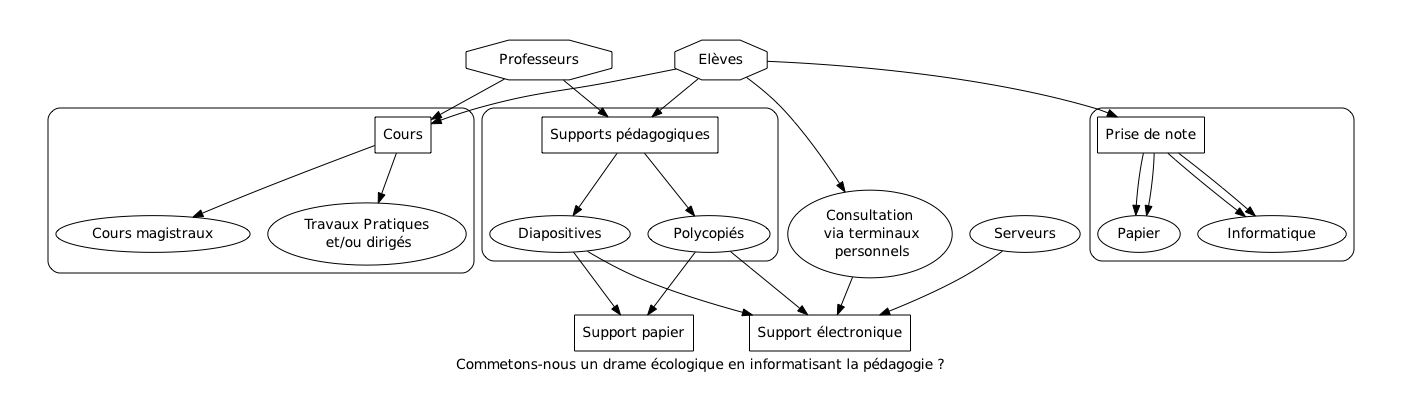
\includegraphics[width=\textwidth]{graphe.png}
  \caption{Graphe des relations au matériel électronique}
  \label{graphe}
  \end{figure}  
\end{frame}


\subsection{Les élèves}

\begin{frame}[label=pagesimple]
  \frametitle{\'Etape 1 : Les élèves}
  Questionnaire envoyé aux élèves de l'\'Ecole.
  \begin{itemize}[<+->]
    \item plus de 300 réponses
    \item une base de données riche et inédite
    \end{itemize}
  \bigskip
  \visible<3->{En déduire le comportement informatique des étudiants}
\end{frame}

\begin{frame} 
  \frametitle{\'Etape 1 : Les élèves}
  \begin{figure}[h!]
  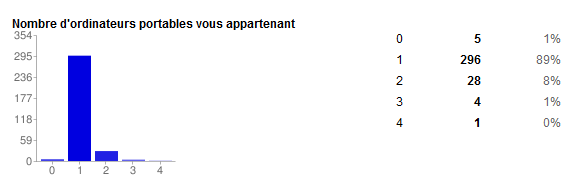
\includegraphics[width=\textwidth]{i1.PNG}
  \caption{Question 1}
  \label{i1}
  \end{figure}
\end{frame}

\begin{frame} 
  \frametitle{\'Etape 1 : Les élèves}
  \begin{figure}[h!]
  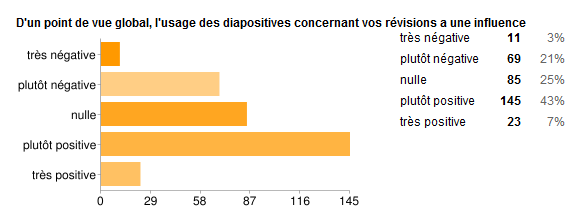
\includegraphics[width=\textwidth]{i2.PNG}
  \caption{Question 2}
  \label{i2}
  \end{figure}
\end{frame}

\begin{frame} 
  \frametitle{\'Etape 1 : Les élèves}
  \begin{figure}[h!]
  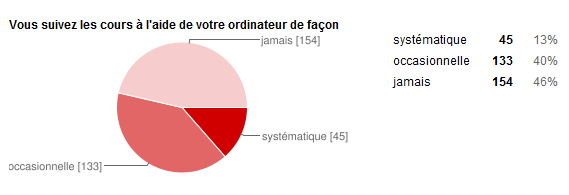
\includegraphics[width=\textwidth]{i3.PNG}
  \caption{Question 3}
  \label{i3}
  \end{figure}
\end{frame}

\begin{frame} 
  \frametitle{\'Etape 1 : Les élèves}
  \begin{figure}[h!]
  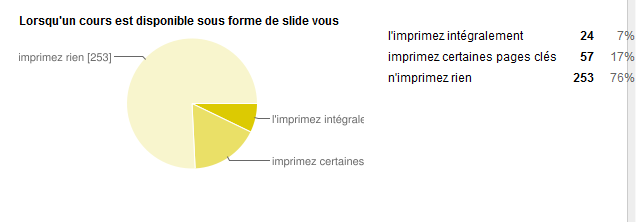
\includegraphics[width=\textwidth]{i4.PNG}
  \caption{Question 4}
  \label{i4}
  \end{figure}
\end{frame}

\begin{frame} 
  \frametitle{\'Etape 1 : Les élèves}
  \begin{figure}[h!]
  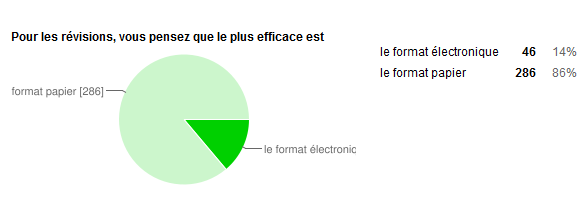
\includegraphics[width=\textwidth]{i5.PNG}
  \caption{Question 5}
  \label{i5}
  \end{figure}
\end{frame}



\subsection{Les enseignants}

\begin{frame}[label=pagesimple]
  \frametitle{\'Etape 2 : Les enseignants}
  Questionnaire envoyé aux enseignants de l'\'Ecole.
  \begin{itemize}[<+->]
    \item plus de 30 réponses
    \item base de données plus réduite
    \end{itemize}
\end{frame}

\begin{frame} 
  \frametitle{\'Etape 2 : Les enseignants}
  \begin{figure}[h!]
  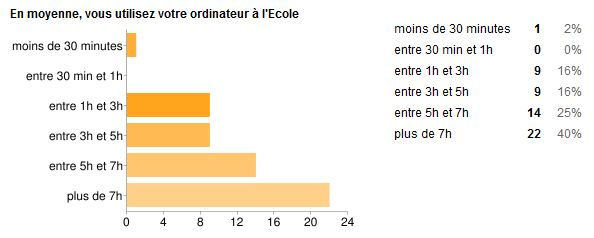
\includegraphics[width=\textwidth]{i6.PNG}
  \caption{Question 1}
  \label{i1}
  \end{figure}
\end{frame}

\begin{frame} 
  \frametitle{\'Etape 2 : Les enseignants}
  \begin{figure}[h!]
  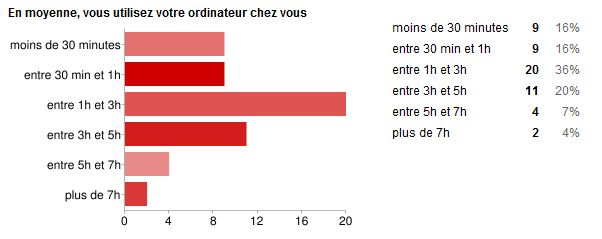
\includegraphics[width=\textwidth]{i7.JPG}
  \caption{Question 2}
  \label{i2}
  \end{figure}
\end{frame}

\begin{frame} 
  \frametitle{\'Etape 2 : Les enseignants}
  \begin{figure}[h!]
  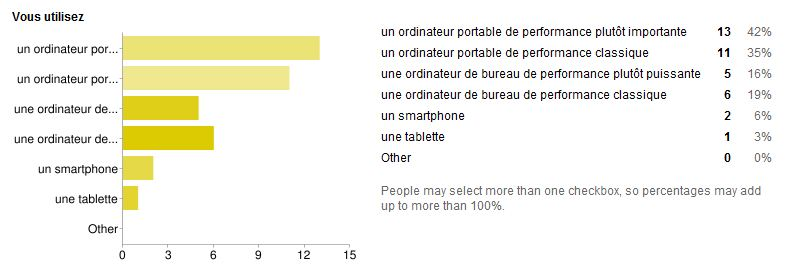
\includegraphics[width=\textwidth]{i8.JPG}
  \caption{Question 3}
  \label{i3}
  \end{figure}
\end{frame}

\begin{frame} 
  \frametitle{\'Etape 2 : Les enseignants}
  \begin{figure}[h!]
  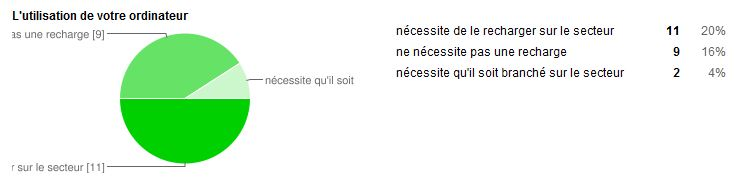
\includegraphics[width=\textwidth]{i9.JPG}
  \caption{Question 4}
  \label{i4}
  \end{figure}
\end{frame}

\begin{frame} 
  \frametitle{\'Etape 2 : Les enseignants}
  \begin{figure}[h!]
  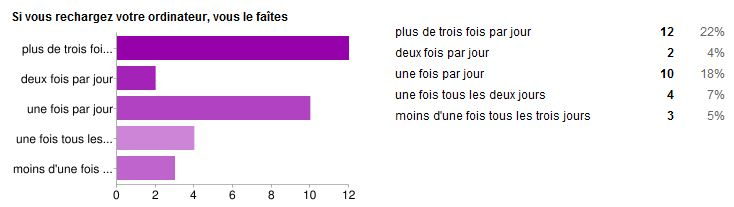
\includegraphics[width=\textwidth]{i10.JPG}
  \caption{Question 5}
  \label{i5}
  \end{figure}
\end{frame}

\begin{frame} 
  \frametitle{\'Etape 2 : Les enseignants}
  \begin{figure}[h!]
  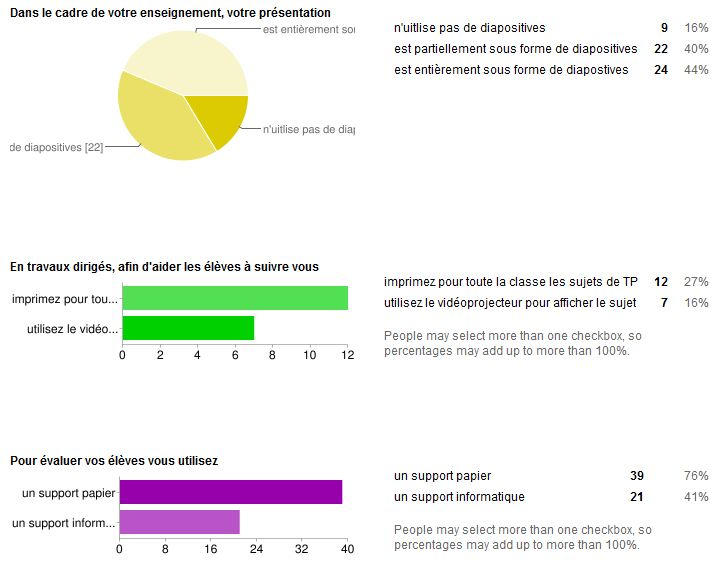
\includegraphics[height=6cm]{i11.JPG}
  \caption{Question 6}
  \label{i5}
  \end{figure}
\end{frame}

\begin{frame} 
  \frametitle{\'Etape 2 : Les enseignants}
  \begin{figure}[h!]
  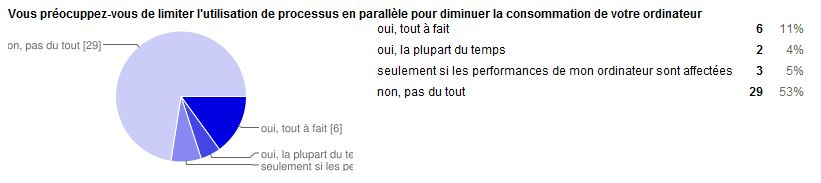
\includegraphics[width=\textwidth]{i12.JPG}
  \caption{Question 7}
  \label{i5}
  \end{figure}
\end{frame}

\begin{frame} 
  \frametitle{\'Etape 2 : Les enseignants}
  \begin{figure}[h!]
  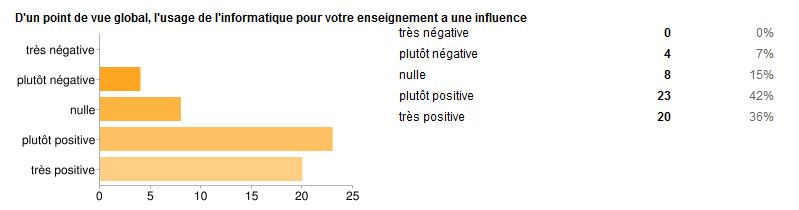
\includegraphics[width=\textwidth]{i13.JPG}
  \caption{Question 8}
  \label{i5}
  \end{figure}
\end{frame}

\subsection{Bilan}
\begin{frame}[label=pagesimple]
  \frametitle{Notre grande enquête}
  \framesubtitle{Conclusion}
  Quelques perspectives :
  \begin{itemize}[<+->]
    \item une appréhension du comportement des utilisateurs,
    \item une anticipation des modifications de l'infrastructure de l'\'Ecole,
    \item une adaptation éventuelle des méthodes pédagogiques.
    \end{itemize}
  \bigskip
\end{frame}

\section{Conclusion}
\begin{frame}{Plan}
  \tableofcontents[sections=\thesection]
\end{frame}

\subsection{GPGPU}

\begin{frame} 
  \frametitle{GPGPU et étude d'un livre}
  \begin{block}{Calcul générique sur un processeur graphique}
     \begin{itemize}[<+->]
       \item Généralisation des solutions de calculs basées sur les processeurs graphiques
       \item Intérêts des processeurs graphiques dans le cadre de l'informatique verte
       \item Inconvénients de telles solutions
     \end{itemize}
   \end{block}
   \begin{block}{\'Etude d'un livre}
     \begin{itemize}[<+->]
       \item Situation actuelle
       \item Mesures à mettre en place
     \end{itemize}
   \end{block} 
\end{frame}


\subsection{Les conseils à suivre}
\begin{frame} 
  \frametitle{Conseils à suivre}
  \framesubtitle{Des gestes quotidiens}
  \begin{block}{Nos conseils}
     \begin{itemize}[<+->]
       \item Éteignez :
       \begin{itemize}
         \item vos haut-parleurs,
         \item votre imprimante,
         \item l'écran,
         \item votre ordianteur (>30min)
       \end{itemize}
     \end{itemize}
  \end{block}   
\end{frame}

\begin{frame} 
  \frametitle{Conseils à suivre}
  \framesubtitle{Des gestes quotidiens}
  \begin{block}{Nos conseils}
     \begin{itemize}[<+->]
       \item Même en veille, un appareil électrique consomme de l'énergie.
       \item Préférez un ordinateur portable à un ordinateur de Bureau.
       \item Éteignez votre modem / box Internet la nuit.
     \end{itemize}
  \end{block}   
\end{frame}



\section{Bibliographie}

\begin{frame} 
\frametitle{Bibliographie}
\begin{thebibliography}{GreenIT}
\bibitem[Ecn]{ecnantes} {Site de l'\'Ecole Centrale de Nantes, \url{http://ec-nantes.fr}\\}

\bibitem[Ind]{indexel} Article sur l'informatique verte via le site indexel.net : regroupe plus d'une vingtaine d'articles sur la Green IT, balayant tous les sujets tels que la réduction de la consommation des ordinateurs à la récupération des déchets électroniques. Les articles sont orginaux et très intéressants. \url{http://www.indexel.net/dossier/informatique-verte.html}\\

\bibitem[Carb]{bilancarbone}Bilan carbone de la mise en ligne d'un article sur le blog du monde.fr  \url{http://bilancarbone.blog.lemonde.fr/}\\

\bibitem[Wiki]{wiki} Article wikipédia sur l'informatique verte \url{http://fr.wikipedia.org/wiki/Green_computing/}\\

\bibitem[GreenIT]{greenit} Site dédié à l'informatique verte \url{http://www.greenit.fr/}\\

\end{thebibliography}
\end{frame}

\begin{frame} 
\frametitle{Bibliographie}
\begin{thebibliography}{GreenIT}


\bibitem[PointA]{pointactu} Quels sont les enjeux de l'informatique verte ? Pointsdactu.org répond à cette question via cet article. \url{http://www.pointsdactu.org/article.php3?id_article=1093}\\

\bibitem[ECOB]{ecob} Article sur le fameux éco-bouton, permettant de mettre en veille votre ordinateur par une simple pression. \url{www.generation-nt.com/eco-button-usb-ecolos-ecologie-actualite-1036961.html}\\

\bibitem[GPU]{gpu} Utilisation d'une carte GPU dans la carte mère [2008] pour résoudre la consommation électrique des ordinateurs. \url{www.pcworld.fr/article/materiel/carte-graphique/nvidia-hybrid-power-la-bonne-idee/88481/?utm_source=matbe&utm_medium=redirect}\\


\end{thebibliography}
\end{frame}

\begin{frame} 
\frametitle{Bibliographie}
\begin{thebibliography}{GreenIT}

\bibitem[CLASS]{classement} Classement \url{http://www.top500.org/list/2010/11/100}\\

\bibitem[GPU2]{GPU2} \url{http://fr.wikipedia.org/wiki/Processeur_graphique}\\

\bibitem[GPGPU]{GPGPU} \url{http://fr.wikipedia.org/wiki/General-Purpose_Processing_on_Graphics_Processing_Units}\\

\bibitem[Green500]{green500} Liste des Green 500 \url{http://www.green500.org/lists/2010/11/top/list.php}\\

\bibitem[Flops]{flops} Article sur la notion d'opétion par seconde \textsf{http://fr.wikipedia.org/wiki/FLOPS}\\

\bibitem[Wiki2]{wiki2} \url{http://fr.wikipedia.org/wiki/Halte_\%C3\%A0_la_croissance_\%3F}\\

\end{thebibliography}
\end{frame}

\begin{frame} 
\frametitle{Bibliographie}
\begin{thebibliography}{GreenIT}

\bibitem[Detic]{Detic} Développement \'Eco-responsable et TIC (DETIC)
\url{http://lesrapports.ladocumentationfrancaise.fr/BRP/094000424/0000.pdf}\\

\bibitem[GreenIT2]{GreenIT2} Olivier PHILIPPOT, \emph{Green IT : Gérez la consommation d'énergie de vos systèmes informatiques Auteur}, DataPro\\

\end{thebibliography}
\end{frame}

\end{document}
